\documentclass{standalone}

\usepackage[latin1]{inputenc}
\usepackage{tikz}

\usetikzlibrary{calc}

% GNUPLOT required
\begin{document}
\pagestyle{empty}


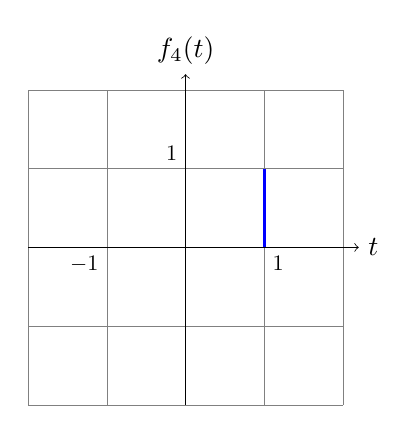
\begin{tikzpicture}[line width=0.3mm]
    \draw[very thin,color=gray] (-2,-2) grid (2,2);
    \draw[->, line width=0.1mm] (-2,0) -- (2.2,0) node[right] {$t$};
    \draw[->, line width=0.1mm] (0,-2) -- (0,2.2) node[above] {$f_{4}(t)$};

	% x(t)
	\draw[very thick,color=blue, domain=-1:0] plot[id=x] function{x+1};
    \draw[very thick,color=blue, domain=0:1] plot[id=x] function{1};
	\draw[very thick,color=blue] (1,0) -- (1,1);


	\foreach \x in {1} {%
    \draw ($(\x,0) + (0,0)$) -- ($(\x,0) + (0,0)$)
        node [below right,scale=0.8] {$\x$};
	}
		\foreach \x in {-1} {%
    \draw ($(\x,0) + (0,0)$) -- ($(\x,0) + (0,0)$)
        node [below left,scale=0.8] {$\x$};
	}
	\foreach \y in {1} {%
    \draw ($(0,\y) + (0,0)$) -- ($(0,\y) + (0,0)$)
        node [above left,scale=0.8] {$\y$};
	}

\end{tikzpicture}


\end{document}
